\documentclass[twocolumn,10pt]{article}

\usepackage{authblk}
\usepackage{bera}
\usepackage[utf8]{inputenc}

% ---------------------------------------------------------------------------
% Packages added by the group
% ---------------------------------------------------------------------------
\usepackage{graphicx}                           % figures, stored in images/
\usepackage{booktabs}                           % tables (\toprule, \midrule, \bottomrule)
\usepackage[font=small,labelfont=bf]{caption}   % compact captions
\usepackage{url}                                % URL of the dataset (footnote)
\usepackage{natbib}                             % \citet{} in the text, \citep{} in brackets
\usepackage{acronym}                            % \ac{} in the text, \acs{} in tables and captions
\usepackage{microtype}                          % fewer bad line breaks in narrow columns

\graphicspath{{images/}}
\raggedbottom                                   % columns are not stretched to the same height
\renewcommand{\bibsection}{}                    % the template already prints "Bibliography"
\hyphenation{Table Figure}                      % no "Ta-ble A1" at the end of a line
\makeatletter
\setlength{\@fptop}{0pt}                        % columns holding only floats start at the top (appendix)
\makeatother

\acrodef{EDA}{Easy Data Augmentation}
\acrodef{LR}{Logistic Regression}
\acrodef{MNB}{Multinomial Naive Bayes}
\acrodef{RQ}{research question}
\acrodef{SVM}{Support Vector Machine}
\acrodef{TFIDF}[TF-IDF]{term frequency--inverse document frequency}

% TITLE
\title{Natural Language - Project report}


% AUTHORS
\author{Group 51: Artur Krystopchuk (104145, 50\%), Filipe Oleacu (106192, 50\%)}
\affil{Instituto Superior Técnico, Universidade de Lisboa}

\begin{document}

\maketitle

\section{Introduction}
\label{sec:intro}

We assign clinical records to one of 12 medical specialties, with 2,662 training and 398 test records adapted from a real Kaggle dataset\footnote{\raggedright\url{https://www.kaggle.com}}. Each record has a \emph{description}, a \emph{sample name}, \emph{keywords} and the \emph{transcription} of the clinical note. The transcription holds most of the text (median 387 words, against \mbox{4--19} for the other fields) but decides the least: identical transcriptions carry different specialties, while the first keyword names the specialty and the section headers (of transcription) reveal the type of document (Section~\ref{sec:analysis}). Hence our \ac{RQ}:

\smallskip
\noindent\textbf{\acs{RQ}:} \emph{Does a short, information-dense input (keywords, sample name, section headers) classify clinical records better than the complete record, and does it still do so when the keywords are missing?}
\smallskip

\noindent Short inputs avoid dilution: in a \ac{TFIDF} vector, normalised to unit length, the first keyword weighs little among the hundreds of words of a complete record. They also carry a risk: a model that relies on the keywords learns a shortcut, copying the first keyword, which fails on the 19.6\% of test records that have no keywords. We therefore compare short and complete inputs with classifiers from \ac{MNB} to a linear \ac{SVM}, and evaluate them separately on records with and without keywords.
% TODO once Section 5 exists: add one sentence with the answer to the RQ ("We find that ...").

\section{Data}
\label{sec:data}

\subsection{Data Analysis}
\label{sec:analysis}

The classes of the 2,662 training records are imbalanced (Table~\ref{tab:classes}): Surgery has 890 records (33.4\%) and Dermatology 25 (0.9\%). Always predicting Surgery reaches 33.4\% accuracy but F1~=~0 for the other 11 classes, failing the shared-task requirement of an F1 of at least 0.25 for every class.

\textbf{O1: one unclosed quote, two kinds of damage.} The 13 lines of the training file without the four ``;'' of a record come from seven truncated lines that hold only a label, an opening quote and the start of a description (the other six are where those quotes close). A CSV reader takes everything up to the closing quote as one field. In four cases, this merges up to 12 records into one description; in the other three, the merged text is cut at exactly 32,759 characters (just under Excel's cell limit) and the rest continues on a new line, read as a record whose label is text (``d is open about\ldots''). Hence \texttt{pandas} returns 2,616 rows and 15 ``labels''. Parsing the file line by line, we drop the seven fragments (their text occurs nowhere else) and rejoin the cut text with the last line, recovering 46 records, having in total 2,662 records.

\textbf{O2: the first keyword is the label} in all 2,219 training records with keywords (``\emph{neurosurgery}, herniated nucleus pulposus, \ldots''), and $ \approx 80\% $ of the test records start with a specialty name; the others have no keywords. Some classes lack keywords far more often than others (Table~\ref{tab:classes}): 66\% of Psychiatry-Psychology records against 4\% of Ophthalmology.

\textbf{O3: the same transcription under several labels.} 58\% of the training records have the same transcription as another record. Together they hold 733 shared transcriptions, and 732 of them appear under different labels; the copies differ only in the label and the first keyword. For example, one ``Anterior Cervical Discectomy'' note appears three times, as Neurosurgery, Orthopedic and Surgery. The reason is that the labels follow two criteria: some name the type of document (84\% of Surgery records are procedure notes, with headers such as ``ANESTHESIA:''; 80\% of Radiology records are imaging reports, with ``IMPRESSION:''), others a body system (Orthopedic, Ophthalmology), so one operation report fits both.

We also found minor noise: in 150 records the keywords end with a website disclaimer (``NOTE: These transcribed medical transcription sample reports\ldots'' inside keywords), 24 records are templates with an empty transcription (``EGD Template - 1''), and names are replaced by placeholders (``I spoke with Dr.~X'').
% Not in the text for space (01_data_analysis.ipynb), useful for Sections 3-6:
% - Test set: 6 records have a single space as keywords; pd.read_csv without .str.strip() counts 72 empty
%   keyword fields instead of 78 (Testing_test_csv.ipynb), which gives 82% instead of 80% (320/398).
%   Delivery/data_analysis.ipynb has the same issue (no_keywords = keywords == "", no .str.strip()): these 6 test
%   rows (11, 160, 165, 230, 304, 371) go to the keyword model with an empty input and are ALL predicted
%   Psychiatry-Psychology; with .str.strip() == "" they go to the text model instead.
% - Transcription length depends on the class (Kruskal-Wallis, p = 1.9e-41): Radiology 230 words, Psych 661.
% - Chi-square test of O2 (missing keywords vs class): chi2 = 285, dof = 11, p = 1.5e-54 (SciPy).
% - O3 in the test set: 60% of the test transcriptions (240) occur in train, and all 210 of them with keywords
%   have ANOTHER label there (e.g. Orthopedic in train -> Surgery in test): memorising training texts fails by
%   construction. A random 80/20 split reproduces this (50% overlap), so our validation splits mirror the test.
% - O3, document types (Table A1, column Type): also 87% of Neurosurgery are procedure notes, 74% of General
%   Medicine and 66% of Psychiatry are consultations.
% - Stop words (for Section 3): the most characteristic words of Surgery are "the, was, then, placed" and of
%   General Medicine "no, history, negative" (log-odds ratio), so we keep stop words.
% - O1 details (raw train.csv): fragments at lines 161, 714, 947, 1088, 2089, 2329, 2394; their quotes close at
%   lines 163, 726, 961, 1096, 2100, 2337, 2395; the cut blocks continue at lines 962, 2101, 2338 (one character
%   is lost at each cut: "wou|d", "|ypothyroidism", "inse|ted"). 32,759 counts each line break as 2 characters
%   (the file uses CRLF); 01_data_analysis.ipynb prints 32,745-32,751 because it counts them as 1.
% - Artefacts in the test set too: disclaimer in 10 keyword fields, 6 keyword fields that hold a single space.
% - Artefacts to clean in train AND test: website disclaimer glued to the keywords (150 / 10 records),
%   ".," = flattened line break, placeholders (Dr. X, XYZ), " - N" suffix of sample names.
% - The header regex of functions.py (used by the models) differs from the one of 01_data_analysis.ipynb
%   (PROCEDURE: 848 vs 776 records); describe the one of functions.py in Section 3.

\subsection{Data Augmentation}
\label{sec:augmentation}

After an 80/20 split, the training part has 712 Surgery records but only 20 Dermatology records. We balance it by adding new versions of random records of each other class until every class has 712 records; validation and test records are never changed.

The new versions are made by \emph{clinical \acs{EDA}}, our adaptation of \acl{EDA}~\citep[\acs{EDA};][]{wei2019eda}\acused{EDA}. \acs{EDA} changes a text with four random word operations; we keep two and adapt them to clinical notes. (i)~\emph{Sentence dropout}: instead of single words, we delete whole sentences, each with probability $p=0.2$, so the remaining sentences keep their meaning (\emph{no fracture} never loses its \emph{no}). (ii)~\emph{Abbreviation replacement}: instead of WordNet synonyms, which cover little medical vocabulary, we swap 30 frequent abbreviations with their full form, or the reverse, each occurrence with $p=0.5$ (MRI $\leftrightarrow$ \emph{magnetic resonance imaging}). We drop random swap and insertion, as they create word sequences that never occur in real notes.


On the complete record (Table~\ref{tab:augmentation}), \ac{MNB} without balancing reaches F1~=~0 for Dermatology, and new rows raise its macro-F1 from 0.18 to 0.53. How the new rows are written matters little: exact copies score like clinical \acs{EDA}, because a new row stays 93\% similar to its original (cosine similarity of their \ac{TFIDF} vectors). We therefore use clinical \acs{EDA} for \ac{MNB}. For the linear models we use class weights instead, which balance the classes without new rows: the error on each record is multiplied by $n/(12\,n_c)$, where $n_c$ is the size of its class and $n$ that of the training part. They score like clinical \acs{EDA} for \ac{LR} (0.57 vs 0.58) and for the \ac{SVM} on the keywords (0.82 for both); only the \ac{SVM} on the complete record gains from the new rows (0.62 vs 0.52), probably because, with four times more rows, its regularisation penalty (set by $C$) weighs less.
% Source: Delivery/data_analysis.ipynb, section "Data Augmentation" (split 42) = Table A2. Not in the text for space:
% - Keywords only: new rows do not remove the shortcut; the lowest F1 stays 0.17 (Psychiatry-Psychology) because
%   the new rows repeat the same keywords, so the validation records without keywords still look alike.
% - For the RQ: even with new rows, the complete record (SVM 0.62) stays far below the keywords alone (0.82).
% - C and p (0.2, 0.5) are not tuned. Old 3-split comparison with SMOTE, undersampling and original EDA:
%   Testing/Manual/02_data_augmentation.ipynb (not delivered).
% IDEA (links 2.2 to the RQ, not implemented): "keyword dropout" = extra copies of training records with the
%   keywords removed. Missing keywords depend on the class (O2: Psychiatry 66%), so a keyword model learns
%   "no keywords -> Psychiatry"; keyword dropout would make one model use the other fields when keywords are
%   missing (an alternative to the two-model routing of the Delivery notebook).

\section{Models}
\label{sec:models}
% PLAN that follows from Sections 1-2 (delete these comments once the section is written).
% Inputs (functions.build_input_variants; headers = functions.extract_headers as HEADER_<NAME> tokens):
%   complete = description + sample_name + transcription + keywords (+ headers)
%   short    = subsets of {keywords, sample_name, description, headers}
% Evidence so far (split 42 only), LinearSVC, accuracy / macro-F1:
%   Delivery: keywords 0.841 / 0.823 | all features 0.480 / 0.522 | all features except transcription 0.792 / 0.764
%   (all features: 0.482 / 0.516 when the notebook runs on Artur's computer, see Table A2; rerun once before the end)
%   03_data_analysis.ipynb (not in Delivery): keywords + transcription 0.497 / 0.535 | keywords + description
%   0.831 / 0.772 | keywords + headers 0.880 / 0.844 | keywords + sample_name 0.889 / 0.864
%   -> with keywords, every long extra field dilutes the label word (first half of the RQ).
%   Without keywords (description + sample_name + headers): SVC 0.356 / 0.404, LR 0.448 / 0.492.
% Models (at least 3; replicable):
%   M1 MNB + TF-IDF + clinical EDA (Section 2.2): the family of the shared-task baseline.
%   M2 LR + TF-IDF word 1-2-grams, class_weight="balanced"; tune C.
%   M3 LinearSVC, same TF-IDF input and class weights; tune C. (No transformer: TinyBERT dropped, see Future Work.)
%   Open half of the RQ (without keywords), Delivery/data_analysis.ipynb, split 42, LR macro-F1: 0.524 with the
%      transcription vs 0.492 without -> here the complete record helps, so the routing's second model reads it.
%   M4 (submission) routing: records with keywords -> LinearSVC on the keywords; records without -> LR on
%      description + sample_name + transcription + headers. Split 42: 0.904 accuracy / 0.883 macro-F1;
%      441/446 right with keywords, 41/87 without (Delivery, Best Model).
%   Reference: rule "first keyword = label" (100% of the training records with keywords, O2).

\section{Experimental Setup}
\label{sec:setup}
% - Data: data/original_train.csv (the professor's train.csv), repaired line by line in Delivery/data_analysis.ipynb;
%   the test set (data/test_no_labels.csv) is only used to write results.txt (398 lines, same order, no header).
% - Split: one stratified 80/20 split (random_state=42), as in Delivery/data_analysis.ipynb; it mirrors the test
%   set (O3). Say "split 42" wherever numbers are given (no mean over splits).
% - Libraries: scikit-learn and pandas as footnotes with their URLs, not as papers (bibliography kept minimal).
% - Metrics: accuracy, macro-F1, lowest per-class F1 (shared task: accuracy > 0.49 and every F1 >= 0.25),
%   each on all validation records AND on those without keywords (17% of train, 20% of test).

\subsection{Parameters/Hyperparameters}
% TF-IDF: word 1-2-grams, lowercase, min_df=2 (term in >= 2 records), sublinear_tf (1 + log tf),
%   max_features=50,000; MNB: alpha=1 (add-one smoothing); LR: C=1, max_iter=2000; LinearSVC: C=0.5;
%   clinical EDA: p_sentence=0.2, p_abbreviation=0.5. Explain each hyperparameter in one clause.

\section{Results}
\label{sec:results}
% - Main table: input (complete ... short) x model x subset (all / with keywords / without keywords).
% - Per-class F1 of the best model; confusion matrix with short class names (as in Table A1): Figure 1.
% - Refer to Figure~\ref{fig:confusion} in the text (template tip). From the figure (Delivery, split 42): 46 of the
%   51 errors are records without keywords (87 records); 23 errors are predictions of General Medicine, all of
%   records without keywords (Cardio-Pulm 7, Gastro 7, Neurology 4, ...). With keywords: 5 errors in 446 records.

\begin{figure}[!t]
\centering
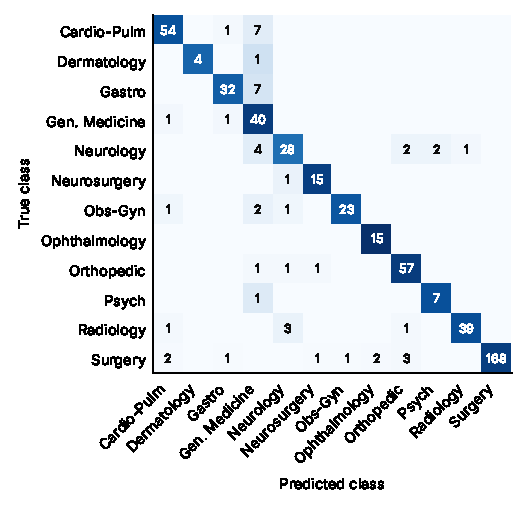
\includegraphics[width=\columnwidth]{confusion_matrix_best_model}
\caption{Confusion matrix of the routing model (\acs{SVM} on the keywords; \acs{LR} on the other fields when the keywords are missing) on the validation part of split 42 (533 records). Rows: true class; columns: predicted class; numbers: records; colour: share of the true class. 46 of the 51 errors are records without keywords, 23 of them predicted as General Medicine.}
\label{fig:confusion}
\end{figure}

\section{Discussion}
\label{sec:discussion}
% - Why does more text hurt? TF-IDF vectors are L2-normalised: in a 400-word record the label keyword is one
%   term among hundreds, and the transcription is shared between labels (O3).
% - Shortcut failure (keywords-only LinearSVC, split 42): Psychiatry-Psychology precision 0.09, recall 1.00,
%   F1 0.17 (Delivery, Testing Only Keywords: lowest F1 0.17).
%   Its 8 records are all found, but 88 records get this label: all 87 validation records without
%   keywords all look alike ("keywords:" and nothing else), and Psychiatry is the class most often without
%   keywords (66%, O2). With the headers added, accuracy on these records rises from 0.08 to 0.32 (03 notebook).
% - Example errors of the routing model (Delivery, Best Model, split 42; all five checked, same predictions):
%   * "Falls at home. Anxiety and depression." appears twice (rows 1503 and 766), true labels Psychiatry and
%     Neurology, both predicted General Medicine: same record, different labels (O3).
%   * "Left heart catheterization, ..." (row 2447): Surgery predicted Cardiovascular-Pulmonary (O3: document
%     type vs organ system). "MRI Brain & MRI C-T spine ..." (row 1725): Radiology predicted Neurology.
%   * With keywords, "surgery, ruptured globe, ..." (row 2635): Surgery predicted Ophthalmology, although the
%     first keyword is the label: the other keywords outweigh it.
% - Answer the RQ explicitly: with keywords / without keywords.

\section{Future Work}
\label{sec:future}
% - Keyword dropout (Section 2.2); a fine-tuned transformer (e.g. TinyBERT) for the records without keywords,
%   reading word order: 34% of the transcriptions exceed 512 words (its limit is 512 tokens) -> keep the head
%   and the tail of each transcription; treat the shared transcriptions (O3) as a multi-label problem.

\section*{Bibliography}
% Template requirement: declare explicitly how LLMs were used. Suggested wording (adapt to what you did):
% "We used Claude (Anthropic) to help draft and edit the text of Sections 1-2 and to review our code; all numbers
%  come from our notebooks, and all analyses and design decisions were checked by the authors."
% (Write it as normal text here, not as a comment.)
% Bibliography kept minimal on purpose: only EDA (wei2019eda), the method we adapt; libraries as footnotes.

\bibliographystyle{apalike}
\bibliography{biblio}
% Template: the bibliography does not count for the 3 pages limit.

% One page at most. Only the first two pages of the paper will be read. The appendix should only contain complementary information.

\clearpage                                      % the appendix starts on its own page (max. one page)
\appendix
\setcounter{figure}{0}
\renewcommand{\thefigure}{A\arabic{figure}}
\setcounter{table}{0}
\renewcommand{\thetable}{A\arabic{table}}

\section*{Appendix A: Extra Figures and Tables}
% Template: maximum one page (it does not count for the 3 pages limit), just extra figures and tables.
% The 3 pages must be understandable without them.

\begin{table}[!ht]
\centering
\footnotesize
\setlength{\tabcolsep}{4pt}
\caption{Training set per class: records ($n$), \% without keywords, \% whose transcription is shared with another record, median words per transcription and main document type (P: procedure, I: imaging or test report, C: consultation) with its \%.}
\label{tab:classes}
\begin{tabular}{@{}lrrrrl@{}}
\toprule
Class          & $n$   & No kw & Shared & Words & Type \\
\midrule
Surgery        & 890   &  7 & 61 & 405 & P 84 \\
Cardio-Pulm    & 308   & 25 & 58 & 358 & P 37 \\
Orthopedic     & 300   & 16 & 71 & 505 & P 60 \\
Radiology      & 222   &  9 & 73 & 230 & I 80 \\
Gen.\ Medicine & 211   & 42 &  8 & 420 & C 74 \\
Gastro         & 195   & 15 & 60 & 285 & P 54 \\
Neurology      & 184   & 27 & 55 & 419 & I 48 \\
Obs-Gyn        & 135   & 17 & 65 & 387 & P 52 \\
Neurosurgery   &  78   & 15 & 92 & 538 & P 87 \\
Ophthalmology  &  73   &  4 & 58 & 323 & P 68 \\
Psych          &  41   & 66 & 20 & 661 & C 66 \\
Dermatology    &  25   & 20 & 48 & 254 & P 44 \\
\midrule
All            & 2,662 & 17 & 58 & 387 & P 52 \\
\bottomrule
\end{tabular}
\end{table}

\begin{table}[!ht]
\centering
\footnotesize
\setlength{\tabcolsep}{3.5pt}
\caption{Balancing on the validation part of split 42: macro-F1 (F1) and lowest per-class F1 (Min). Complete record: all fields and the section headers, as \acs{TFIDF} of word 1--2-grams. \acs{MNB} has no class weights; on the new rows, class weights change nothing, as every class has 712 records.}
\label{tab:augmentation}
\begin{tabular}{@{}lcccccc@{}}
\toprule
                     & \multicolumn{2}{c}{\acs{MNB}} & \multicolumn{2}{c}{\acs{LR}} & \multicolumn{2}{c}{\acs{SVM}} \\
\cmidrule(lr){2-3}\cmidrule(lr){4-5}\cmidrule(l){6-7}
Balancing            & F1   & Min  & F1   & Min  & F1   & Min  \\
\midrule
\multicolumn{7}{@{}l}{\emph{Complete record}} \\
None                 & .183 & .000 & --   & --   & --   & --   \\
Class weights        & --   & --   & .571 & .364 & .516 & .154 \\
Exact copies         & .527 & .312 & --   & --   & --   & --   \\
Clinical \acs{EDA}   & .532 & .293 & .581 & .256 & .620 & .211 \\
\midrule
\multicolumn{7}{@{}l}{\emph{Keywords only}} \\
None                 & .296 & .000 & --   & --   & --   & --   \\
Class weights        & --   & --   & .764 & .167 & .823 & .167 \\
Clinical \acs{EDA}   & .456 & .165 & .778 & .167 & .822 & .167 \\
\bottomrule
\end{tabular}
\end{table}

\begin{figure}[!ht]
\centering
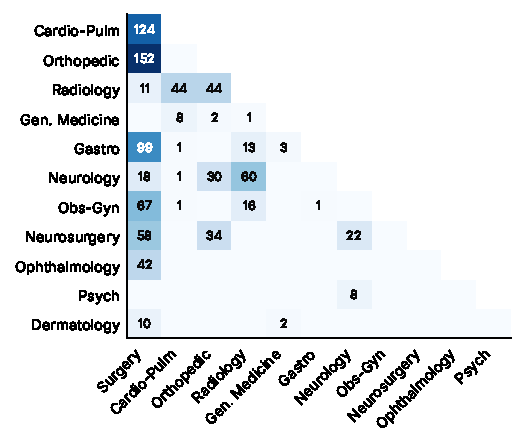
\includegraphics[width=\columnwidth]{shared_reports_between_classes}
\caption{Identical transcriptions with different labels, per pair of classes (training set, O3): each cell counts the transcriptions that appear, word for word, under both classes; e.g., 152 transcriptions appear both as Surgery and as Orthopedic.}
\label{fig:shared}
\end{figure}

\clearpage                                      % added: keeps the appendix page intact (remove with the tips)
\section{Evaluation and tips (remove this section before submission)}

Scores by section:
\begin{itemize}
\item (1.5) Introduction: beyond the classification task itself, \textbf{explicitly} identify the research question your group wants to answer. For instance: how does classical machine learning compare to current language models on clinical text? Which data augmentation strategy is most effective for highly imbalanced medical datasets? This research question should guide your model choices, your experimental setup, and your discussion. It defines the \textbf{story of the paper}. The remaining sections of the paper should be read as an attempt to answer it.
\item (1.5) Data Analysis: describe the dataset (class distribution and relevant statistics); provide at least 2 concrete observations about patterns or anomalies you found by looking at the data. Generic descriptions score zero.
\item (2.0) Data Augmentation: you should do some kind of data augmentation. Clearly describe your strategy.
\item (4.0) Models: clearly describe the models you built and the choices you made, considering the research question you have identified previously (you should describe at least 3 models) (1.0). When describing your models, keep replicability in mind (1.0): would someone be able to reproduce your results just by reading this section? We will also reward creativity (2.0): did you explore different approaches and make thoughtful choices, or did you simply run code you found online?
\item (1.0) Experimental Setup: provide clear information regarding the used datasets, splits (which result in your own test set(s)), evaluation metrics used and hyperparameters (if applicable).
\item (1.5) Results: provide the results of your best models, and also results by label of your best model. You should also present a comprehensive confusion matrix of one of your models (not necessarily the best one). The given test set (test\_no\_labels.txt) should ****only**** be used to generate the file results.txt.
\item (3.0) Discussion: show us that you have properly analysed the dataset and the obtained outputs (not just by looking at statistics or confusion matrices). Try to explain the most common errors. Present and discuss at least 3 concrete examples of misclassified instances from your own test set (include the text excerpt, the predicted label, the correct label, and your interpretation). Generic statements score zero. Also, explain how results align with the research question you have identified in the introduction.
\item (0.5) Future Work: if more time was given, explain what you would do to improve your system, considering the research question identified in the introduction.
\item (1.0) References: Identify all papers, external sources, and pre-trained models used; also explicitly declare how have you used LLMs.
\end{itemize}
Tips:
\begin{itemize}
\item Label figures and tables.
\item Use the correct quotation marks in Latex (``bla-bla'').
\item If you use a figure or table, refer to it.
\item If you say things such as ``The dataset is unbalanced'', explain why (facts).
\item Use formal English (so, no ``it's'', ``they're'', etc.).
\item If you mention a hyperparameter, explain it (briefly).
\item If you use an acronym, use it consistently (check how to do it in latex).
\item Use labels that are easy to be read in the Confusion Matrix.
\item Cite your sources (papers) or add footnotes with URLs for computational resources.
\item Do not use subjective adjectives (e.g.: amazing work, nice concept, ...). This is science.
\end{itemize}


\end{document}

 \item{How the project will be evaluated}
\begin{itemize}
\item (1.5) General quality of the paper: are the proposed methods sound? Clearness, zero typos, illustrative examples, pictures and figures, etc.
\item (1.5) Replicability: if we wanted to replicate your results, just by reading the paper, would we be able to do it?
\item (2.0) The creativity of your approach: you just limited yourself to run a code you found somewhere or you tried different approaches?
\item (1.0) References: identify all external sources, libraries, and pre-trained models used; also explicitly declare how have you used LLMs.
